\subsubsection{Implement network security}

\textbf{Azure Virtual Network} \\
Design best practices:
\begin{enumerate}
\item Minimise conflicts. \textit{Ensure non-overlapping address spaces. The VNet address space (CIDR block) should not overlap with your organization's other network ranges.}
\item Keep a reserve space. \textit{Reserve some of the address space of the VNet.}
\item Minimise management overhead. \textit{Create a few large VNets, rather than multiple small VNets.}
\item Secure it. \textit{Secure your VNet using Network Security Groups (NSGs)}.
\end{enumerate}

Communication: \\
All resources in a VNet can communicate outbound to the internet, by default. You can communicate inbound to a resource by assigning a public IP address or a public Load Balancer. When using only an internal Standard Load Balancer, outbound connectivity is not available until you define how you want outbound connections to work with an instance-level public IP or a public Load Balancer.

The communication options of Azure resources are:
\begin{itemize}
\item Virtual network: \textit{Deploy VMs, and other Azure resources to a virtual network, such as Azure App Service Environments, the Azure Kubernetes Service (AKS), or Azure Virtual Machine Scale Sets.}
\item Through a virtual network service endpoint: \textit{Extend your virtual network private address space and the identity of your virtual network to Azure service resources, such as Azure Storage accounts and Azure SQL databases, over a direct connection. Service endpoints allow you to secure your critical Azure service resources to only a virtual network.}
\item VNet Peering: \textit{Connect virtual networks to each other, enabling resources in either virtual network to communicate with each other, using virtual network peering. The virtual networks you connect can be in the same, or different, Azure regions.}
\end{itemize}

The communication options for on-premise resources are:
\begin{itemize}
\item Point-to-site virtual private network (VPN): \textit{Established between a virtual network and a single computer in your network. Each computer must configure an individual connection. Intended for developers, as it requires few adjustments to existing network. The communication is encrypted.}
\item Site-to-site VPN: \textit{Established between on-premises VPN device and an Azure VPN Gateway in a virtual network. This connection type enables any on-premises resource that you authorize to access a virtual network. The communication is encrypted.}
\item Azure ExpressRoute: \textit{Established between your network and Azure, through an ExpressRoute partner. This connection is private. Traffic does not go over the internet.}
\end{itemize}

You can filter network traffic between subnets using either or both of the following options:
\begin{itemize}
\item Security groups: \textit{Network security groups and application security groups can contain multiple inbound and outbound security rules that enable you to filter traffic to and from resources by source and destination IP address, port, and protocol.}
\item Network virtual appliances:\textit{A network virtual appliance is a VM that performs a network function, such as a firewall, WAN optimization, or other network function.}
\end{itemize}

Azure routes traffic between subnets, connected virtual networks, on-premises networks, and the Internet, by default. You can implement either or both of the following options to override the default routes Azure creates:
\begin{itemize}
\item Route tables: \textit{Custom route tables with routes that control where traffic is routed to for each subnet.}
\item Border gateway protocol (BGP) routes: \textit{Connect the virtual network to the on-premises network using an Azure VPN Gateway or ExpressRoute connection, you can propagate your on-premises BGP routes to your virtual networks. }
\end{itemize}

\textbf{Network Security Groups} \\
Security rules in network security groups enable you to filter the type of network traffic that can flow in and out of virtual network subnets and network interfaces.

A network security group (NSG) contains a list of security rules that allow or deny network traffic to resources connected to Azure Virtual Networks (VNet). NSGs can be associated to subnets, individual VMs (classic), or individual network interfaces (NIC) attached to VMs (Resource Manager).  When an NSG is associated to a subnet, the rules apply to all resources connected to the subnet. Traffic can further be restricted by also associating an NSG to a VM or NIC.

\begin{figure}[!h]
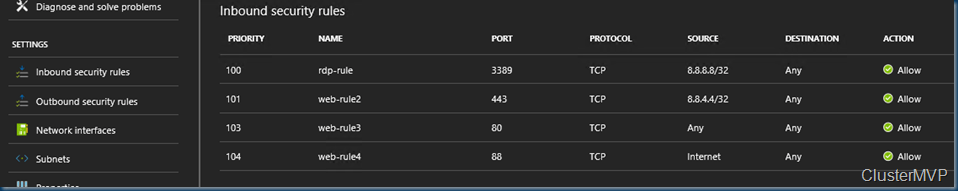
\includegraphics[width=1\textwidth]{platform-network-rules.png}
\caption{List of inbound security rules}
\end{figure}